\subsection{The Aftermath: Denial, Rage, and Possibly Murder}

The Pythagoreans didn’t take this well. According to legend, Hippasus --- the guy who discovered irrational numbers --- was drowned at sea for revealing the truth.

Did this actually happen? Probably not. But it says a lot about how much they hated the idea.  

Unfortunately for them, the truth doesn’t care about your philosophy. The discovery of irrational numbers shattered the idea that the universe was built on neat, whole-number ratios.  

\textbf{Mathematics was no longer just about counting and measuring. It was about confronting the unknown.}  

And it was only going to get weirder from here.

\begin{figure}[H]
\centering
\begin{tikzpicture}[every node/.style={font=\footnotesize}]

% Panel 1 — Nervous follower confesses
\comicpanel{0}{4}
  {Follower}
  {}
  {\textbf{Follower:} So... um... Hippasus says \(\sqrt{2}\) isn’t a ratio. He says it just… keeps going.}
  {(0,-0.5)}

% Panel 2 — Senior Pythagorean processing
\comicpanel{6.5}{4}
  {Pythagorean}
  {}
  {\textbf{Pythagorean:} That can’t be right.  
Tell him to double-check with nicer fractions.}
  {(0,-0.5)}

% Panel 3 — Another Pythagorean enters with "news"
\comicpanel{0}{0}
  {Messenger}
  {}
  {\textbf{Messenger:} Uh… Hippasus had an accident.  
Fell off a boat. Mid-proof. Tragic.}
  {(0,0.8)}

% Panel 4 — Stoic onlooker delivers punchline
\comicpanel{6.5}{0}
  {Onlooker}
  {}
  {\textbf{Onlooker:} It’s always the followers who vanish mysteriously. Never the leaders.}
  {(0,0.8)}

\end{tikzpicture}
\caption{The discovery of irrational numbers didn’t just change math; it also thinned the research team.}
\end{figure}

